% !TEX root = DesignDocument.tex


\chapter{User Documentation}

\section{User Guide}


\section{Installation Guide}
The following is the steps to install the DanceSoft software on a users machine:

\bf Step 1: \rm
	The first thing a user needs to do is make sure that a valid version of Python 3 can run on their system, if you already have python 3 installed on your machine please skip to step 2.
	The most recent version of Python 3 can be found on \url{https://www.python.org/downloads/} the user can then click on the download link and download a python zip file that is compatible with the operating system being used by the user.
	Follow the instruction on the install, one the install is complete the python files should be located in your local drive unless the user specified a different directory during install. A user has several ways of confirming that python installed correctly on their system. If the user is  with the command prompt they can run the Python 3 command to confirm successful installation. If the user would like to confirm using non-command line, the user can go to the python 3 file on their drive and run the Python.exe file. If a command window appears then the user has successfully installed python and can proceed to step 2.
	
\begin{figure}
  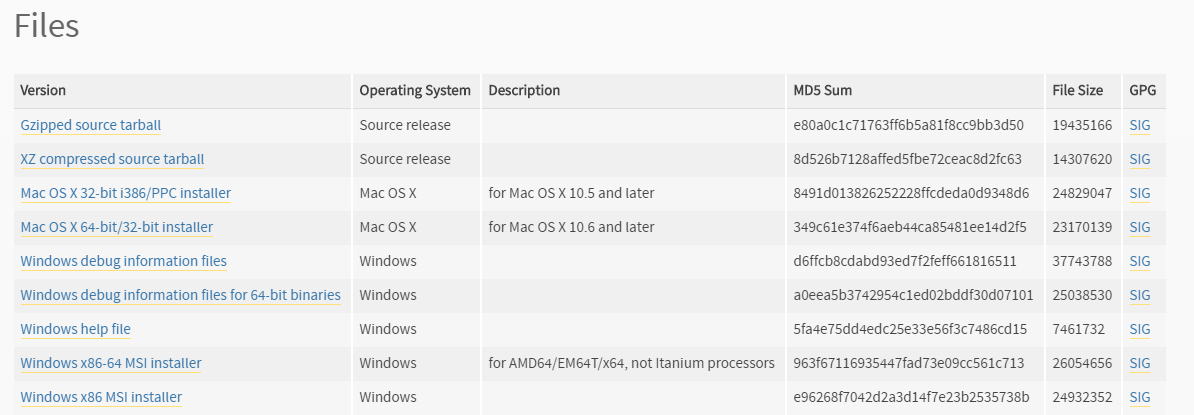
\includegraphics[width=\linewidth]{pics/pythonFiles.png}
  \caption{Python zip files}
  \label{fig:User doc: python files}
\end{figure}

\bf Step 2: \rm
	The next step is to install the PyQt libraries and the designer so the user can run the scripts containing PyQt code. There are several versions of PyQt, the version the DanceSoft team used was PyQt4. PyQt4 can be downloaded from \url{https://www.riverbankcomputing.com/software/pyqt/download}, one there the user can select the zip file that goes with their operating system. The website also provides stable windows installers if the user is running a windows system. If the installer is used the libraries will automaticlly be stored in the site-packages sub-directory of the python folder and the user should be able to start using PyQt libraries
	If the user is not running windows, they can download and use the brew facility to easily install the need files. If the user runs \bf brew install PyQt --with-python3 \rm from the OS X command line the system should automaticly install the needed files.
	 Otherwise the user will need to download the snippets from \url{https://www.riverbankcomputing.com/software/pyqt/download} and install the PyQt libraries in the site-packages folder.
	 
\bf Step 3: \rm
	The last major install a user will need to do before using the software is the MySQL database software neccisary to use the SQL components of the DanceSoft project.
	MySQL can be installed by following the download instructions on \url{https://www.mysql.com/downloads/} and downloading the free version of the software. This installer will install all the tools needed to mulnipulate and use the database directly if necessary.
	
\\	
	
The user should now have all the needed tools installed to run the DanceSoft Software.
	 
	


%% \newpage  %%  if needed ...
%\section{Programmer Manual}

